\documentclass[a4paper,12pt,twoside,openright]{report}
\usepackage[titletoc]{appendix}
\usepackage{textcomp}
\usepackage[pdftex]{color,graphics}
\usepackage{amssymb}
\usepackage{verbatim}
\usepackage{graphicx}
\usepackage{graphics}
\usepackage{amsmath}
\usepackage{rotating}
\usepackage{setspace}
\usepackage{multirow}
\usepackage{array}
\usepackage{hhline}
\usepackage[labelfont={bf}, margin=0.5cm]{caption}
\usepackage{pdflscape}
\usepackage{subcaption}
\usepackage{caption}
\usepackage{xspace}
\usepackage{float}
\usepackage{placeins}
\usepackage{etoolbox}
\usepackage{xkeyval}[2006/11/18]
\usepackage{datetime}
\usepackage[a4paper,inner=2.5cm,outer=1.5cm,top=2.5cm,bottom=2.5cm,pdftex]{geometry}
\usepackage{emptypage}
\usepackage{hyperref}

\hypersetup{
	linktocpage,
    colorlinks = true,
	linkcolor = blue,
	citecolor = red
}

\usepackage{fancyhdr}
\fancyfoot{}
\pagestyle{fancy}
\fancyhead[LO]{\leftmark}
\fancyhead[RE]{\rightmark}
\fancyhead[RO,LE]{\thepage}

\renewcommand{\textfraction}{.05}
\renewcommand{\floatpagefraction}{.40}

\newcommand{\gr}{$\gamma$-ray\xspace}
\newcommand{\grs}{$\gamma$-rays\xspace}

\usepackage{lipsum}% just to automatically generate text

\makeatletter
\newcommand\ackname{Acknowledgements}
\if@titlepage
  \newenvironment{acknowledgements}{%
      \titlepage
      \null\vfil
      \@beginparpenalty\@lowpenalty
      \begin{center}%
        \bfseries \ackname
        \@endparpenalty\@M
      \end{center}}%
     {\par\vfil\null\endtitlepage}
\else
  \newenvironment{acknowledgements}{%
      \if@twocolumn
        \section*{\abstractname}%
      \else
        \small
        \begin{center}%
          {\bfseries \ackname\vspace{-.5em}\vspace{\z@}}%
        \end{center}%
        \quotation
      \fi}
      {\if@twocolumn\else\endquotation\fi}
\fi
\makeatother

\newdateformat{monthyeardate}{%
  \monthname[\THEMONTH], \THEYEAR}

%\textheight 24cm
%\textwidth 16.5cm
%\topmargin -1cm
%\oddsidemargin  0cm
%\evensidemargin 0cm
%\flushbottom

%\usepackage{etoolbox}
%\patchcmd{\chapter}{\thispagestyle{plain}}{\thispagestyle{fancy}}{}{}

\setlength{\headheight}{15pt}


\begin{document}


\setcounter{secnumdepth}{3}
\setcounter{tocdepth}{3}

%\doublespace

\pagenumbering{roman}

\begin{titlepage}

\begin{center}

\textbf{\Huge Upgrades to the }

\vspace{3mm}

\textbf{\Huge Fluorescence Detectors of the}

\vspace{3mm}

\textbf{\Huge Pierre Auger Observatory} 

\vspace{3cm}


\includegraphics[width=0.3\textwidth]{pix/UoA_col_vert.png}

\vspace{3cm}


\textbf{\large Tristan William Sudholz} \\
\vspace{0.4cm}
\large School of Physical Sciences \\
\vspace{0.1cm}
\large University of Adelaide

\vspace{1.5cm}
\large This dissertation is submitted for the degree of \\
\vspace{0.2cm}
\textit{\large Doctor of Philosophy}
\vspace{2.5cm}

\monthyeardate\today

\end{center}

\end{titlepage}

%\chapter*{Declaration}

I, Tristan William Sudholz, certify that this work contains no material which has been accepted for the award of any other 
degree or diploma in any university or other tertiary institution and, to the best of my knowledge and
belief, contains no material previously published or written by another person, except where due
reference has been made in the text. In addition, I certify that no part of this work will, in the future,
be used in a submission for any other degree or diploma in any university or other tertiary institution 
without the prior approval of the University of Adelaide and where applicable, any partner institution
responsible for the joint-award of this degree.

I give consent to this copy of my thesis, when deposited in the University Library, being made
available for loan and photocopying, subject to the provisions of the Copyright Act 1968.

I also give permission for the digital version of my thesis to be made available on the web, via the
University’s digital research repository, the Library catalogue and also through web search engines,
unless permission has been granted by the University to restrict access for a period of time. 

\vspace{2cm}

\line(1,0){150}

\vspace{1cm}

Tristan William Sudholz
\chapter*{Abstract}


%
\chapter*{Acknowledgements}



\tableofcontents
%\listoffigures
%\listoftables

\chapter*{Nomenclature}

\addcontentsline{toc}{chapter}{Nomenclature}

\begin{tabular}{p{8em} p{30em}}
PAO & Pierre Auger Observatory \\
EAS & Extensive Air Shower \\
NSB & Night Sky Background \\
PE & Photo-electron \\
FD & Fluorescence Detector \\
SD & Surface Detector \\
PMT & Photomultiplier Tube \\
FLT & First Level Trigger
\end{tabular}

\chapter*{Introduction}\label{Ch:Intro}
\markright{Introduction}
\addcontentsline{toc}{chapter}{Introduction}
\pagenumbering{arabic}

\begin{itemize}
\item Define Cosmics Rays.
\item The origins of the highest energy cosmic-rays still unknown.
\item First detection by Pierre Auger in 1937 and the current detector looking at theses energies is the Pierre Auger Observatory.
\item Hybrid experiment containing both surface detectors and fluorescence detectors
\item Surface detector has nearly 100\% up-time while the fluorescence detectors only have 15\% up-time.
\item **** Proposal to extend the fluorescence detector up-time. To achieve this will have to operator while the moon is above the horizon. This will increase the level NSB and will have the PMTs run under a reduced gain to compensate. ****
\item Photomultiplier Tubes are used as pixels within the camera of the fluorescence detectors and  the aim of these thesis is to quantify the characteristics of the PMT under the reduced gain and increased.
\item Outline a Summary of each chapter.
\end{itemize}


Cosmic-rays are particles that originate outside of the Earth atmosphere. These particles can be photons, hadronic or leptonic in nature [ref?]. In this thesis, when mentioning cosmic-rays I will mean the hadronic component unless specified otherwise. Cosmic-rays have been measurement over a large range of energies (over 6 decades in energy) and it has many interesting features have been observed in this energy spectrum. One of the longest running mysteries is what happens at the highest energy. Since the first detection of extensive air showers by Pierre Auger in 1937 [ref], many different experiments have endeavoured to solve this mystery. The Pierre Auger Observatory [ref] is currently in operation to observe cosmic-rays at the highest energies. 

The Pierre Auger Observatory is a hybrid experiment consisting of both surface detectors and fluorescence detectors. (Outline location) The surface detector has a nearly 100\% operation up-time {ref} while the fluorescence detectors only 15\% operation up-time [ref]. (Outline how PAO detects cosmic-rays, just need a brief summary).

A current proposal to extend the fluorescence detector operation up-time. Extended up-time would be beneficial as the fluorescence detectors image the entire extensive air shower and would increase the number of showers observed through out yearly observation. To achieve the extended operation the fluorescence detectors would have to operated while the moon is above the horizon. While the moon is up, this would increased the Night Sky Background level and to compensate the Photomultiplier Tubes acting as the camera pixels would have to be run under reduced gain. 

The aim of this thesis is to quantify the characteristics of the Photomultiplier Tubes operating under this reduced gain and outline any operation strategies. Outline of each chapter is as follows:

\begin{itemize}
\item  Chapter \ref{Ch:Cosmic-rays}: Cosmic-rays

Does this work as a new line

\item Chapter \ref{Ch:CR_Detection}: Detection of Cosmic-Rays

Add text here

\item Chapter \ref{Ch:PAO}: The Pierre Auger Observatory

Add text here

\item Chapter \ref{Ch:SelectEff} : EAS Selection Efficiency with Increased NSB 

Add text here

\item Chapter \ref{Ch:PMTCharacter} : Quantifying Characteristics of the FD PMT 

Add text here

\item Chapter \ref{Ch:CompSimPMT} : Computer Simulation of the FD PMT 

Add text here

\item Chapter \ref{Ch:GainVariance} : Measuring Gain Variance of the FD PMT with CalA data 

Add text here

\item Chapter \ref{Ch:LabPMTshift} : Laboratory Simulation of FD Shifts

Add text here

\item Chapter \ref{Ch:CloudCuts} : Effectiveness of Cloud Camera Cuts

Add text here

\item Chapter \ref{Ch:Conclusion}: Conclusion 

Future Work


\end{itemize}
\chapter[Cosmic-Rays]{\centering Cosmic-Rays \\}\label{Ch:Cosmic-rays}

\section{History of Cosmic-Rays}

First detection of ionizing radiation. 

1785: Coulomb found that 
electroscopes can spontaneously 
discharge by the action of the air 
and not by defective insulation

1835: Faraday confirms the 
observation by Coulomb, with 
better insulation technology

1879: Crookes measures that the 
speed of discharge of an 
electroscope decreased when 
pressure was reduced 

\section{Energy Spectrum and Mass composition}

\begin{figure}[hp]
\centering
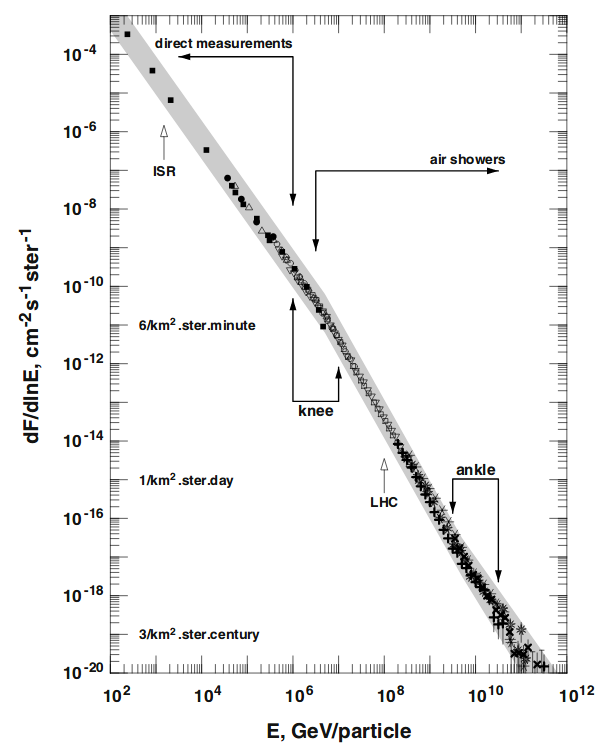
\includegraphics[width=\textwidth]{chapters/pix/CosmicRay_Spectrum.png}
\caption{Measured energy spectrum of cosmic-rays from 100 GeV up to the highest detected energy.}
\label{fig:CR_Spectrum}
\end{figure}

Cosmic-rays have been detected over a large range of energies from GeV (10$^9$ \ eV) to above EeV (10$^18$ \ eV). Spectrum in Figure \ref{fig:CR_Spectrum} shows the break at the knee and ankle and which type of experiments are most suited to measurement each part. Cosmic-ray spectrum starts out at E$^{-2}$ \ and can be as steep as E$^{-2.7}$ at the highest energies.

Cosmic-rays can consist of protons to iron. 

\section{Production Method and Sources}

Supernova explosions 

AGN jets

other energetic processes

dark matter annihilations.
\chapter{Detections of Cosmic-Rays}\label{Ch:CR_Detection}

\section{Extensive Air Showers}

Use Earth's atmosphere as an interaction medium.
Primary particle interacts with the molecules in the atmosphere to produce a cascade of secondary particles. This cascade of particles is referred to as an Extensive Air Shower (EAS).
Hadronic primaries can produce pions, muons and other stuff.
Mixture of a hadronic core with an electromagnetic component from the decay of $\pi^{0}$.

Shower profile has particles produced until energy on individual secondary particles drop below the ionization threshold. Therefore the shower will reach a point of maximum particle number then will drop off.

\section{Fluorescence Production}

The charge particles of EAS interact with the nitrogen molecules in the atmosphere. This interaction turns the nitrogen molecule dipole like and when the nitrogen returns to a ground state, a photon is emitted. This emitted photon is termed fluorescence light. Fluorescence light is can be emitted isotropically and typically in the UV band (between 300 and 400 nm). *** Show wavelength profile ***


\section{Atmospheric Effects}




\section{Detectors and History}

Early Experiments:

Volcano Ranch

Haverah Park

SUGAR

Yakutsk array is located in Russia and has been operating in different forms since 1967. The array reached a maximum collecting area of 17 km$^2$ around 1990. Recently it has been reconfigured to have a collection area of 8 km$^2$ to study lower energy cosmic-rays.

Akeno Gaint Air Shower Array (AGASA) is located in Tokyo, Japan. Operating at an average altitude of 667 m above sea level from 1990 to 2004. The array consist of over one hundred scintillator detectors covering 100 km$^2$ ***check this***. The timing measurements and data collection is achieved via interconnected optical fibers.

The Fly's Eye was the first successful air fluorescence detector operating from 1981 to 1993 at the Dugway Proving Grounds in Utah, USA. Fly's Eye achieved a time averaged aperture of about 100 km$^2$sr at the highest energies, considering it only operated on clear moonless nights. 

HiRes improved on the Fly's Eye design by advancing resolution and sensitivity, This was achieved by increasing the telescope effective mirror area to 3.8 m$^2$ and reducing the camera pixel angular diameter to 1\textdegree. 
\chapter{Pierre Auger Observatory}\label{Ch:PAO}


Science Goals

Location

\section{Hybrid Detector}

\subsection{Surface Detector}

\subsection{Fluorescence Detector}

\section{Communication System and CDAS}

\section{Event Reconstruction}

\subsection{Surface Detector}

\subsection{Fluorescence Detector}

\section{Enhancements and future upgrades}
\chapter[EAS Selection Efficiency with Increased NSB]{\centering Extensive Air Shower Selection Efficiency with Increased \\ Night Sky Background \\}\label{Ch:SelectEff}


%Selection Efficiency of EAS under increased NSB
%\begin{itemize}
%\item Smearing real data with extra noise
%\item Simulating EAS with an increased NSB
%\item Talk about differences in smearing and simulating EAS (different triggering conditions)
%\item Energy and Xmas resolution and bias
%\item Rp bias
%\item differences in track length
%\end{itemize}

\section{Motivation}

The FD shifts are typically organised for night with the illuminated fraction of the moon less then 70\% and can be operated longer than 3 hours of moon below the horizon. The Fd telescope shutters are then opened when the sun is below -18\textdegree of the horizon (astronomical twilight), the average variance of the camera PMTs less then 100 ADC$^2$ and individual PMTs less then 2000 ADC$^2$. Two calculations where done by the collaboration to estimate the theoretical up time of the FD's. Before 2012 the theoretical calculations looked like:

\begin{table}[h]
\centering
\begin{tabular}{c c}
Theoretical up time & 22\% \\
Loss due to short nights ($<$ 3 hrs) & -2\% \\
Loss due to bad weather or fails & -5\% \\ \hline \hline
Total measurement time & 15\% 
\end{tabular}
\end{table}

For context the measured ADC$^2$ for typically observed Night Sky Background (NSB) with no moon, quarter moon and full moon/twilight is:
\begin{table}[h]
\centering
\begin{tabular}{c c c}
\hline\hline
Condition & $\sigma^2$ [ADC$^2$] & I$_{\mathrm{a}}$ [$\mu$A] \\ \hline\hline
no moon & 25 & 0.5 \\
quarter moon & 250 & 5 \\
full moon/twilight & 2500 & 50 \\ \hline\hline
\end{tabular}
\end{table}

These values are measured under the standard operation of the FD's. Further within this thesis I will investigate lower the gain on the PMTs to reduce the variance and current that their under. A lower current when observing under moonlight would help make sure that the PMT lifespans are not changed by the increased in NSB.

The signal that the FD's observe is AC coupled, which means the mean signal of the NSB is zero. Instead the variance around zero is calculated andis directly proportional to the fluctuations in the NSB. The average value of the NSB measured by POA at Malargue is:
\begin{equation}
\sigma^2 \sim 25 \ \mathrm{ADC}^2
\end{equation}
The variance in ADC$^2$ can be converted into photons seen at the aperture by using:
\begin{eqnarray}
\sigma^2_{pe} &=& [\sigma^2_{\mathrm{ADC}}]^{\mathrm{sky}} \ / \ \mathrm{A}^2_{\mathrm{G}} \label{eq:simgaPE} \\
\mathrm{n}_{\mathrm{ph}} &=& \frac{\sigma^2_{pe}}{(1 + \mathrm{V}_{\mathrm{G}})} \label{eq:numPhoton}
\end{eqnarray}
where $\sigma_{pe}$ is the standard deviation of the photo-electron count, n$_{\mathrm{ph}}$ is the photon count and A$_{\mathrm{G}}$ is equal to:
\begin{equation}\label{eq:abs_gain}
\mathrm{A}_{\mathrm{G}} = \frac{1}{\mathrm{C}_{\mathrm{FD}}.\mathrm{f}.\mathrm{Q}}
\end{equation}
where
\begin{itemize}
\item[] A$_{\mathrm{G}}$ is the absolute gain (ADC/photo-electron)
\item[] $\mathrm{C}_{\mathrm{FD}}$ is the FD pixel calibration constant.
\item[] Q is the Quantum efficiency of the PMT.
\item[] f is the efficiency if the telescope optics.
\end{itemize}

/*------ \textbf{Find reference to number below} ------*/

Assuming typical measured values for C$_{\mathrm{FD}}$, Q and f shown in:
\begin{table}[h]
\begin{center}
\begin{tabular}{|c|c|}
\hline
C$_{\mathrm{FD}}$ & 4.5 photons/ADC \\
\hline
Q & 0.29 \\
\hline
f & 0.465 \\
\hline
\end{tabular} 
\end{center}
\caption{} 
\end{table} \label{tab:CFD_Q_F}

Therefore A$_{\mathrm{G}}$ can be calculated from Eq. \ref{eq:abs_gain} and using the values from Table \ref{tab:CFD_Q_F}. If $\sigma^2_{\mathrm{ADC}}$ = 25 ADC$^2$, through the calculations n$_{\mathrm{ph}}$ = 23 photons / 100 ns. The calculations to work out the RMS$_{\mathrm{ph}}$ from the measured variance in ADC$^2$ is as follows:
\begin{equation}
\mathrm{RMS}_{\mathrm{ph}} = \mathrm{C}_{\mathrm{FD}} \times \sqrt{\mathrm{ADC}^2}
\end{equation}
From all of the equations stated above I have outlined a table showing the expected photon count at the aperture per 100 ns from the measured variance (ADC$^2$ / 100 ns).
\begin{center}
\begin{tabular}{| c | c | c | c |}
\hline \hline
\textbf{Variance} & \multirow{2}{*}{\textbf{log$_{10}$(V/ADC$^2$)}} & \multirow{2}{*}{\textbf{Photons/100 ns}} & \textbf{RMS} \\
\textbf{(ADC$^2$ / 100 ns)} & & & \textbf{(Photons/100 ns)} \\
\hline \hline
25 & 1.40 & 22.7 & 22.5 \\
\hline
178 & 2.25 & 161.4 & 60 \\
\hline
259 & 2.40 & 226.7 & 71.2 \\
\hline
1000 & 3.00 & 907.0 & 142.3 \\
\hline
\end{tabular}
\end{center}


- Need graph of expected variance in ADC$^2$ for the moon above the horizon for different phases.

- Want to increase the duty cycle of FD by measuring EAS under moonlight. Most likely observe under quarter to half moon. This will increased the NSB upto a factor of 10.

- The aim of increasing the duty cycle of FD is too measure more EAS at the highest energy band ($> 10^{19.5}$ eV).

- Need more statistics at highest energy band to complement SD measurements.


\section{Selection Efficiency}

I investigated evaluating increasing the NSB by different factors on event reconstruction seen the FD's through a couple of different methods. The main increase of NSB will from observing while the moon is above the horizon. The two methods involved simulating increased NSB on measured data and with simulating. The measured data had increased noise introduced across the entire signal trace and I have labelled as the smearing method.

Selection Efficiency for the two methods are calculated via:
\begin{equation}
\mathrm{Efficiency} = \mathrm{N}_{\mathrm{Selected}} / \mathrm{N}_{\mathrm{total}}
\end{equation}
where for the Smearing method N$_{\mathrm{total}}$ is the total number of measured EAS events at standard NSB levels and N$_{\mathrm{Selected}}$ is the number of events after being reconstructed and passing the quality cuts with the increased NSB. For the simulations, N$_{\mathrm{total}}$ is the total number of simulated events before \textbf{need to check whether its the number of simulations before triggering or number of triggered events at standard NSB. Pretty sure the comparison is done with no. of simulated event at standard NSB}.

Smearing method involves taking the raw fluorescence telescope EAS shower events that would passed reconstruction and quality cuts and adding addition variance in ADC$^2$ equivalent to an increased NSB from moonlight to the FD pixel signal traces. The shower events are then reconstructed and passed through the same quality cuts. This a repartition of a similar method that M. Unger had preformed in \textbf{2012}. \textbf{Also need to refer to the study done by Brue and Andrew Smith around 1999}. This was done so a deeper analysis could be preformed to understand the underlying mechanics. 

The simulations were done using the simulation modules for the FD's within the $\overline{\mathrm{Off}}$\underline{Line} analysis programs. The EAS profiles were generated within CONEX and the original showers were generated through CORSIKA. The NSB was added to the EAS profiles before the FD are triggered. A hybrid trigger is used to involve the SD but the SD is simulated in a simple way just to get a simulated core position.

The smearing method was originally used as a proof of concept to show that EAS showers could still be reconstructed with the increased NSB. The limitation was that EAS were used that already triggered the FD's normally. The full simulation using CONEX showers was used to full test trigger conditions through to reconstruction. The simulations are not an 100\% accurate representation of the POA array so that will introduce some differences too.


\begin{figure}[!hp]
\centering
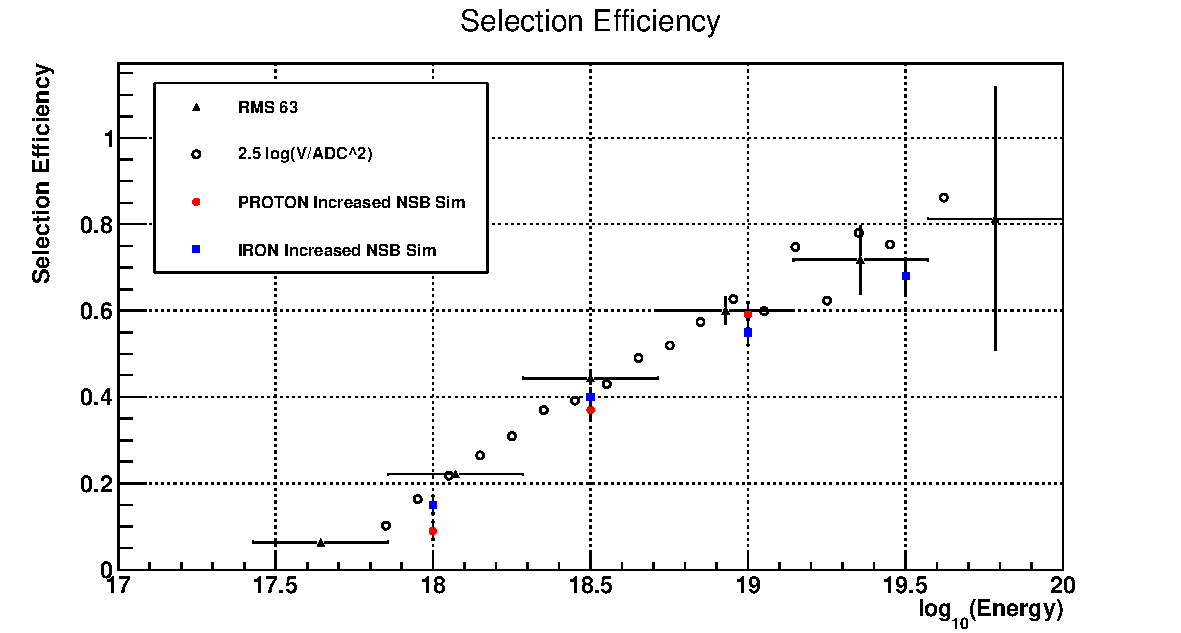
\includegraphics[width=\textwidth]{chapters/graphs/SelectionEff/SelectionEff_errorbars_10timesNSB.pdf}
\caption{Selection Efficiency plot containing data from both the Smearing method and simulated showers. These results are compared to the work done by M. Unger.}
\end{figure}

\section{Resolution and Bias}

To further evaluate the effects of increasing the NSB on the quality of the reconstructed EAS data, I look at the resolution and bias of both the reconstructed energy and reconstructed Xmax. A quick reminder that Xmax is the measurement of the brightest part of the shower relating to the maximum number of particles produced. For the smearing method the energy and Xmax bias is comparing to the measured data taken at standard NSB levels to the reconstructed with the increased NSB levels. For the simulations the energy and Xmax bias can be calculated using the true energy and Xmax values used to generate each EAS profile.

The trend of the energy resolution for both methods is that as the energy of the EAS event increases the bias decreases. This was expected as the energy of the shower increases the brighter and longer the track that is observed. A brighter and longer track allows for a better reconstruction.

- Need to find out what's a good bias value for energy and Xmax.

the energy and Xamx bias is calcualted via:
\begin{eqnarray}
\Delta \mathrm{E} &=& \frac{\mathrm{E}_{\mathrm{recon}} - \mathrm{E}_{\mathrm{true}}}{\mathrm{E}_{\mathrm{true}}}  \label{eq:energybias_sim} \\
\Delta \mathrm{E} &=& \frac{\mathrm{E}_{\mathrm{IncreasedNSB}} - \mathrm{E}_{\mathrm{StandardNSB}}}{\mathrm{E}_{\mathrm{StandardNSB}}} \label{eq:energybias_data} \\
\Delta \mathrm{Xmax} &=& \mathrm{Xmax}_{\mathrm{recon}} - \mathrm{Xmax}_{\mathrm{true}} \label{eq:xmaxbias_sim} \\
\Delta \mathrm{Xmax} &=& \mathrm{Xmax}_{\mathrm{IncreasedNSB}} - \mathrm{Xmax}_{\mathrm{StandardNSB}}\label{eq:xmaxbias_data}
\end{eqnarray}
Eq. \ref{eq:energybias_sim} and Eq. \ref{eq:xmaxbias_sim} are used on the simulated data sets while Eq. \ref{eq:energybias_data} and Eq. \ref{eq:xmaxbias_data} is used on the smeared data set.

The energy and Xmax resolution is calculated via:
\begin{eqnarray}
\sigma_{\mathrm{res}} &=& \left( \frac{1}{\mathrm{N}} \sum \frac{1}{\sigma^2_i} \right)^{1/2}
\end{eqnarray}


\begin{figure}
\centering
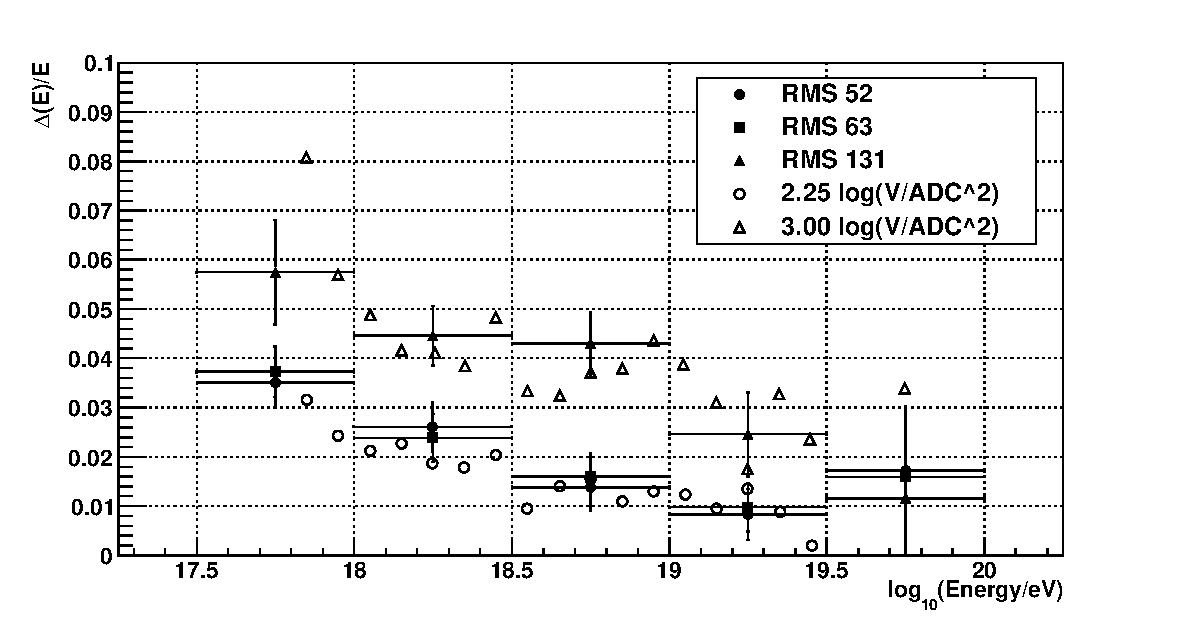
\includegraphics[width=\textwidth]{chapters/graphs/SelectionEff/Smearing_RealData_EnergyBias.pdf}
\caption{Energy Bias using Smearing Method.}
\vspace{3mm}
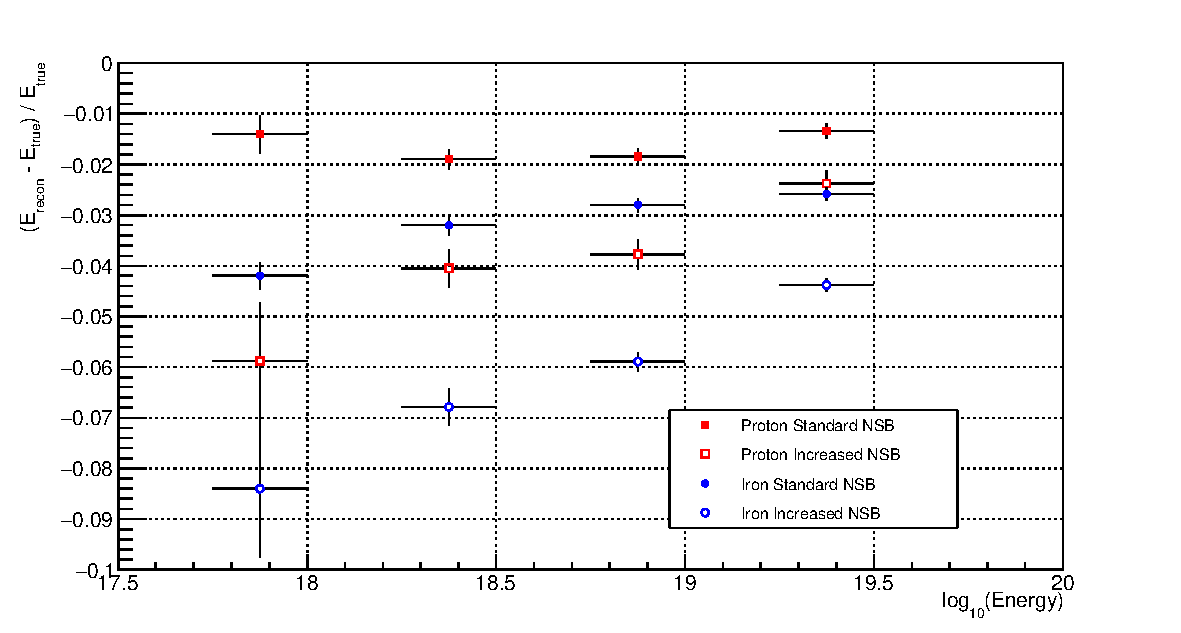
\includegraphics[width=\textwidth]{chapters/graphs/SelectionEff/Simulation_ProtonIron_EnergyBias.pdf}
\caption{Energy Bias using simulated data.}
\end{figure}

\begin{figure}
\centering
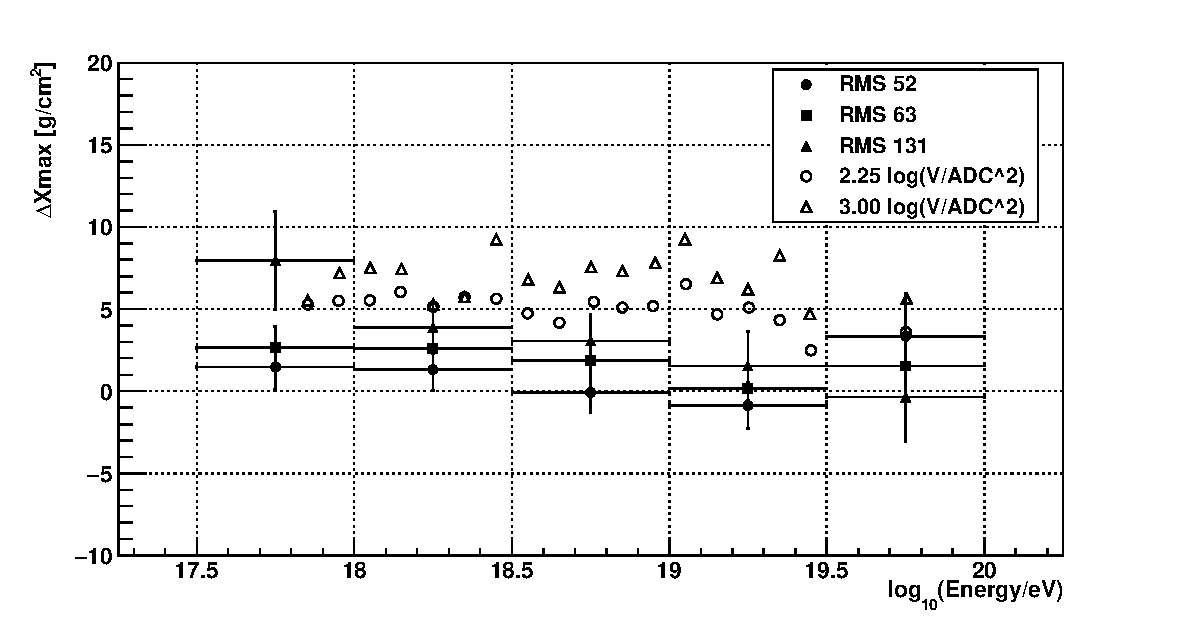
\includegraphics[width=\textwidth]{chapters/graphs/SelectionEff/Smearing_RealData_XmaxBias.pdf}
\caption{Xmax Bias using Smearing Method.}
\vspace{3mm}
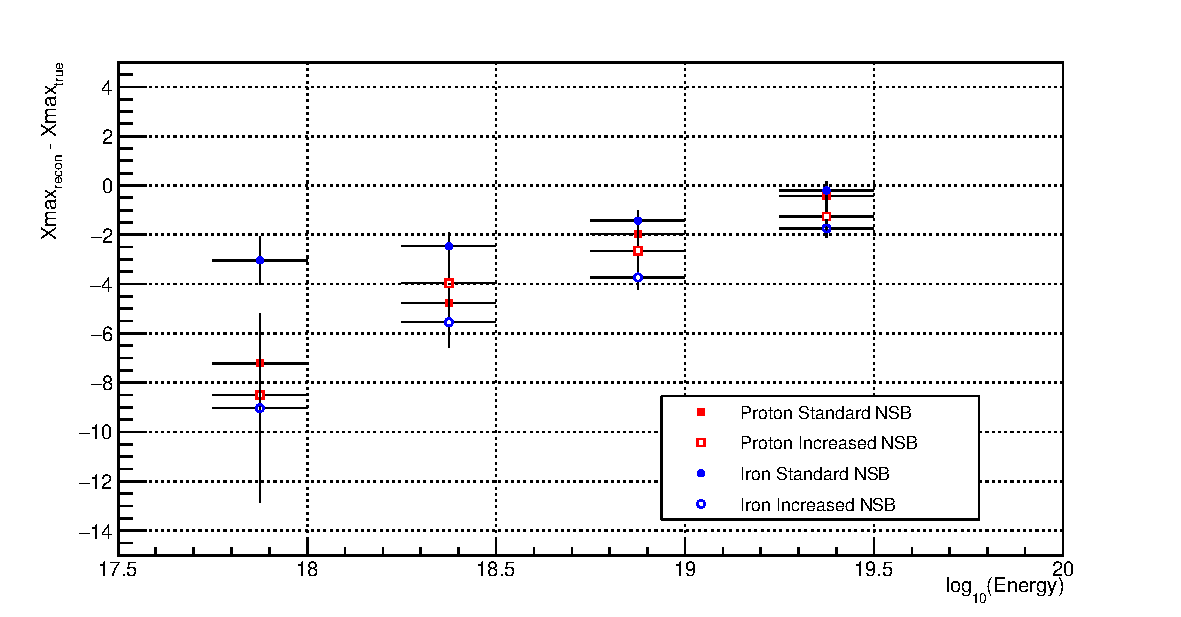
\includegraphics[width=\textwidth]{chapters/graphs/SelectionEff/Simulation_ProtonIron_XmaxBias.pdf}
\caption{Xmax Bias using simulated data.}
\end{figure}

\begin{figure}
\centering
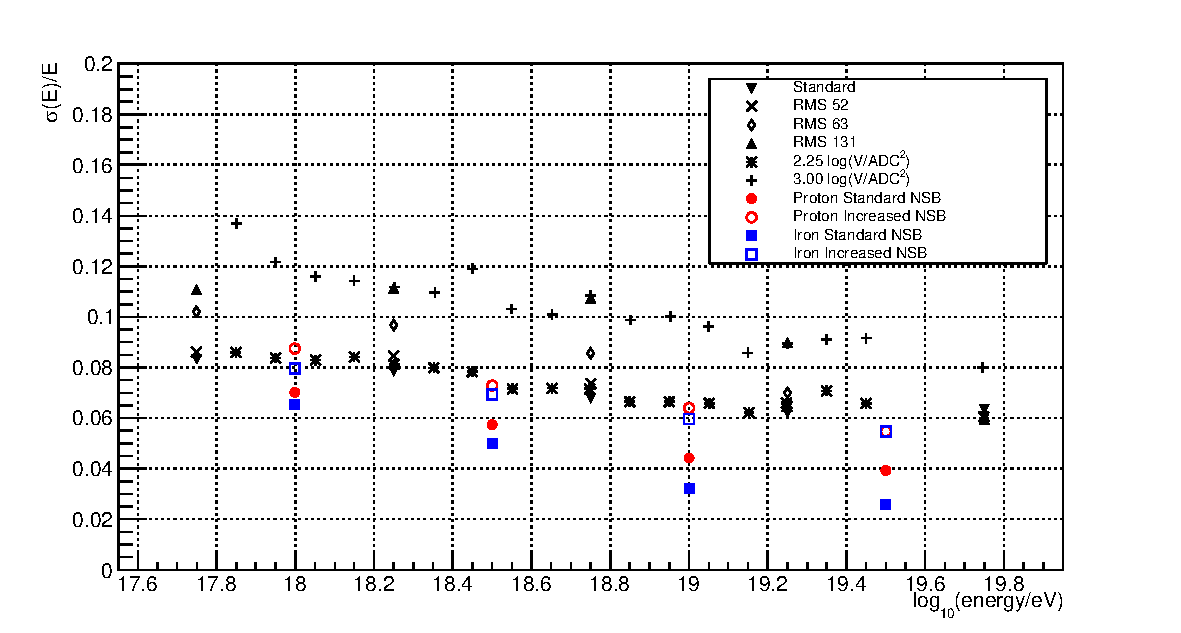
\includegraphics[width=\textwidth]{chapters/graphs/SelectionEff/Combined_EnergyRes_All.pdf}
\caption{Energy Resolution using both Smearing Method data and simulated showers.}
\vspace{3mm}
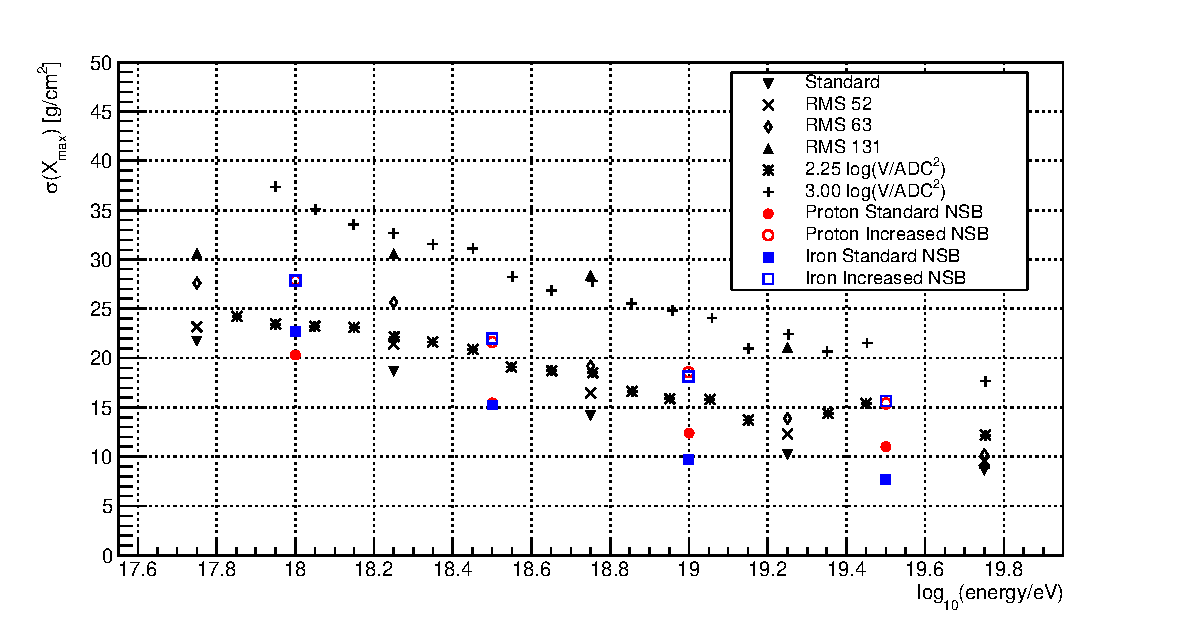
\includegraphics[width=\textwidth]{chapters/graphs/SelectionEff/Combined_XmaxRes_All.pdf}
\caption{Xmax Resolution using both Smearing Method data and simulated showers.}
\end{figure}

\subsection{Comparing Simulated Data to Real Data}

\textbf{Think about where to locate this section.}

Comparing the simulated data with real data. Checking to make sure that the simulation data is a good representation of reality. Looking at the Xmax distribution there is no need for a direction comparison as I only simulated proton and iron primaries and was not concern with have a particular mixtures. The other parameter I checked was the zenith angle distribution, distance to Xmax and distance to the shower axis (R$_{\mathrm{P}}$). The simulated profiles have similar shapes when both histograms are normalised to area of 1. For zenith angle distribution I simulated the EAS events upto a zenith angle of 60\textdegree so that the reason for the cut-off in the simulated data.

\begin{figure}
\centering
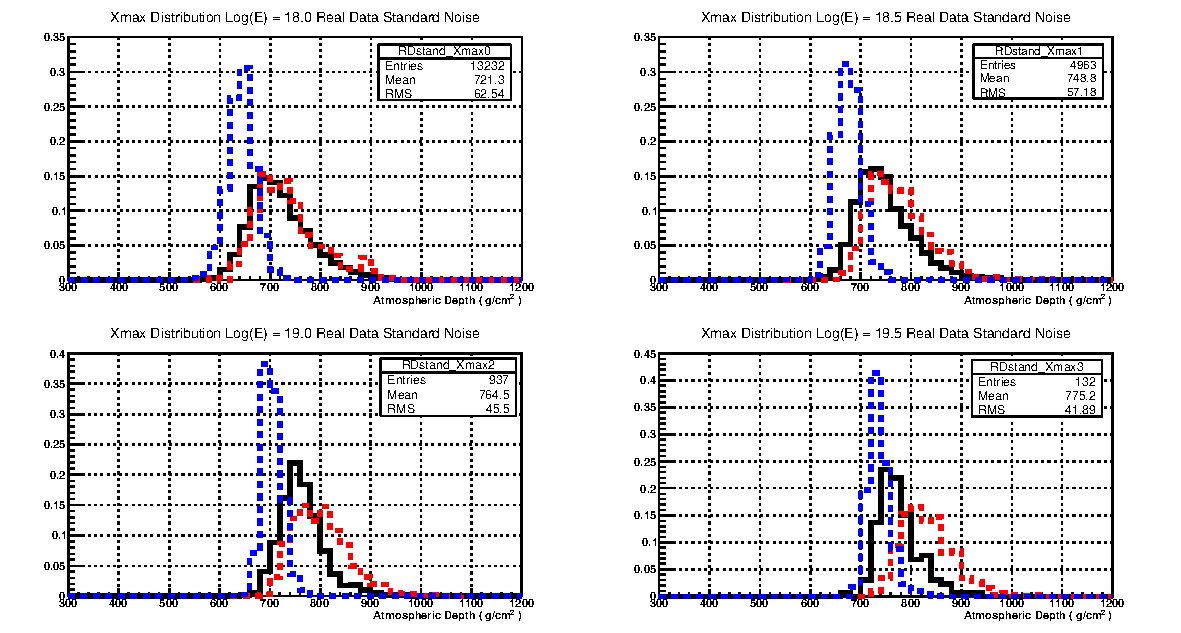
\includegraphics[width=\textwidth]{chapters/graphs/SelectionEff/RealDataAndSim_XmaxDistComp.pdf}
\caption{Distribution of Xmax with Real Data and simulation of proton and iron showers.}
\vspace{3mm}
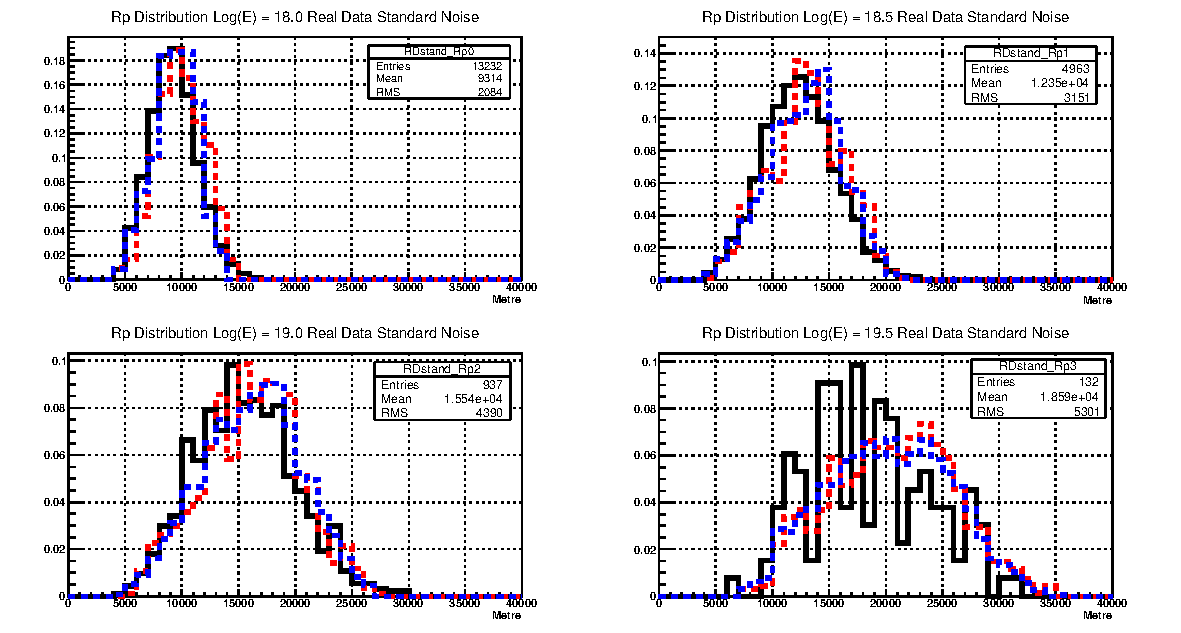
\includegraphics[width=\textwidth]{chapters/graphs/SelectionEff/RealDataAndSim_RpDistComp.pdf}
\caption{Distribution of Rp with Real Data and simulation of proton and iron showers.}
\end{figure}

\begin{figure}
\centering
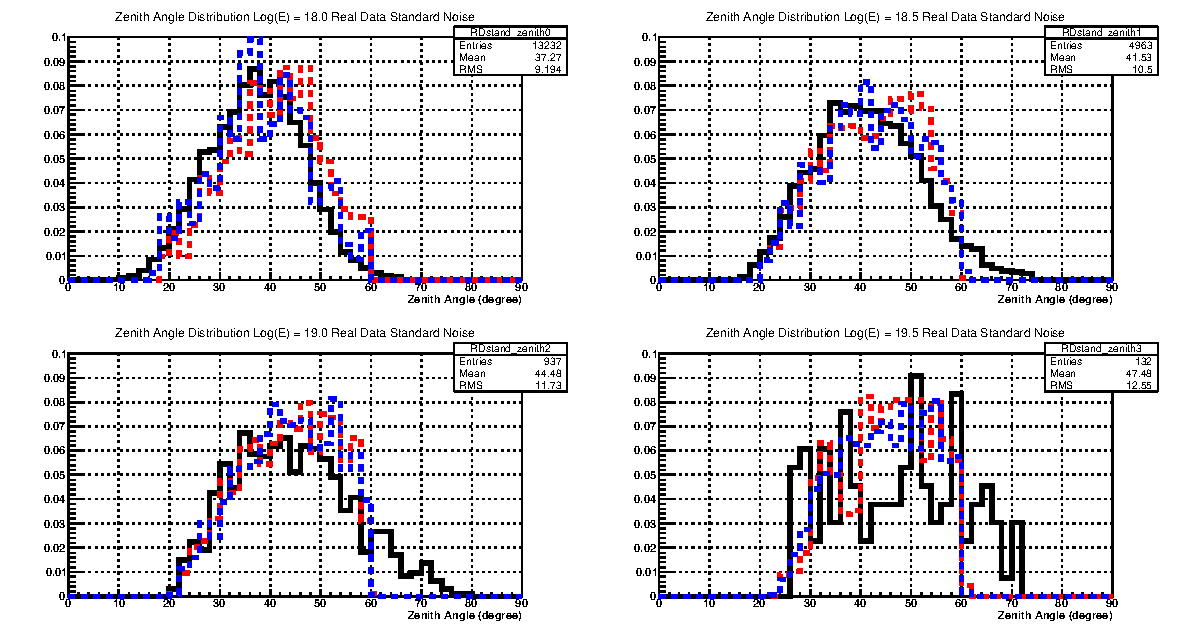
\includegraphics[width=\textwidth]{chapters/graphs/SelectionEff/RealDataAndSim_ZenithDistComp.pdf}
\caption{Distribution of Zenith angle with Real Data and simulation of proton and iron showers.}
\vspace{3mm}
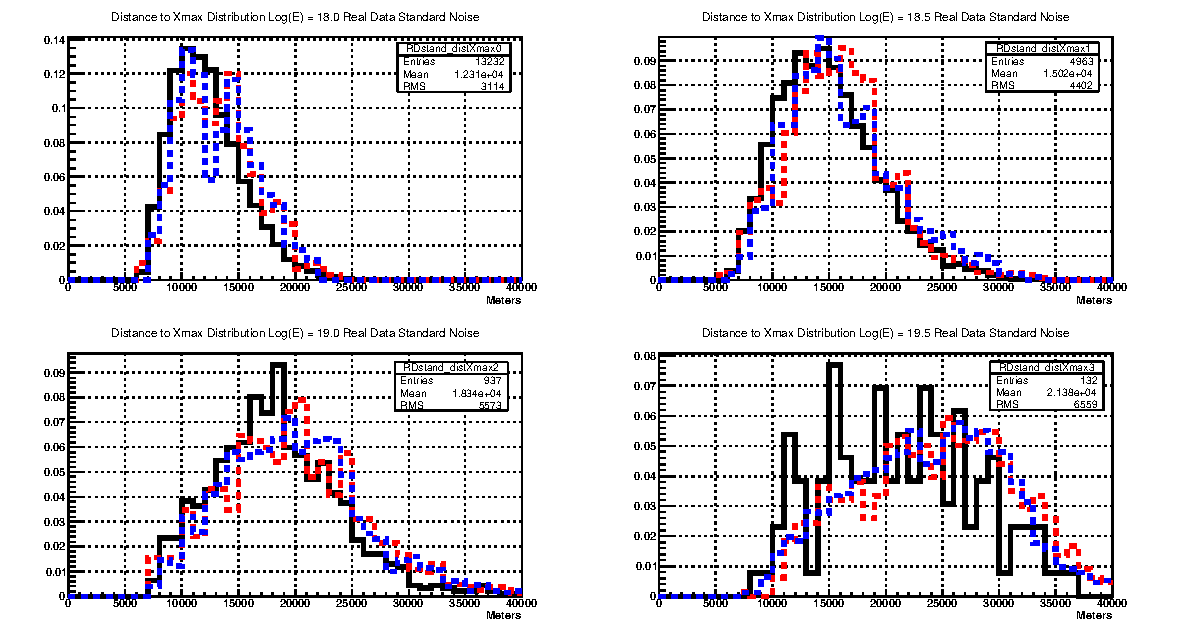
\includegraphics[width=\textwidth]{chapters/graphs/SelectionEff/RealDataAndSim_DistToXmaxDistComp.pdf}
\caption{Distribution of Distance to Xmax with Real Data and simulation of proton and iron showers.}
\end{figure}

\section{EAS Track Length in the FD's}

One other parameter that was investigate was the shower track length observed by the FD's. It was expected that as the NSB increased the average observed shower track length would decrease. For both the smearing and simulation this trend was observed by not in a significant way. This is shown in Fig. \ref{fig:TrackLength_Smearing} and Fig. \ref{fig:TrackLength_Sim}.  There was a thought about trying to extended track length into the noisy pixels as it would be known that would be photons observed at the start and end of the track. The measured data shows that this is not needed as not much of the track is lost with increased NSB. Especially at the highest energy bins where the most interest lays. 

\begin{figure}
\centering
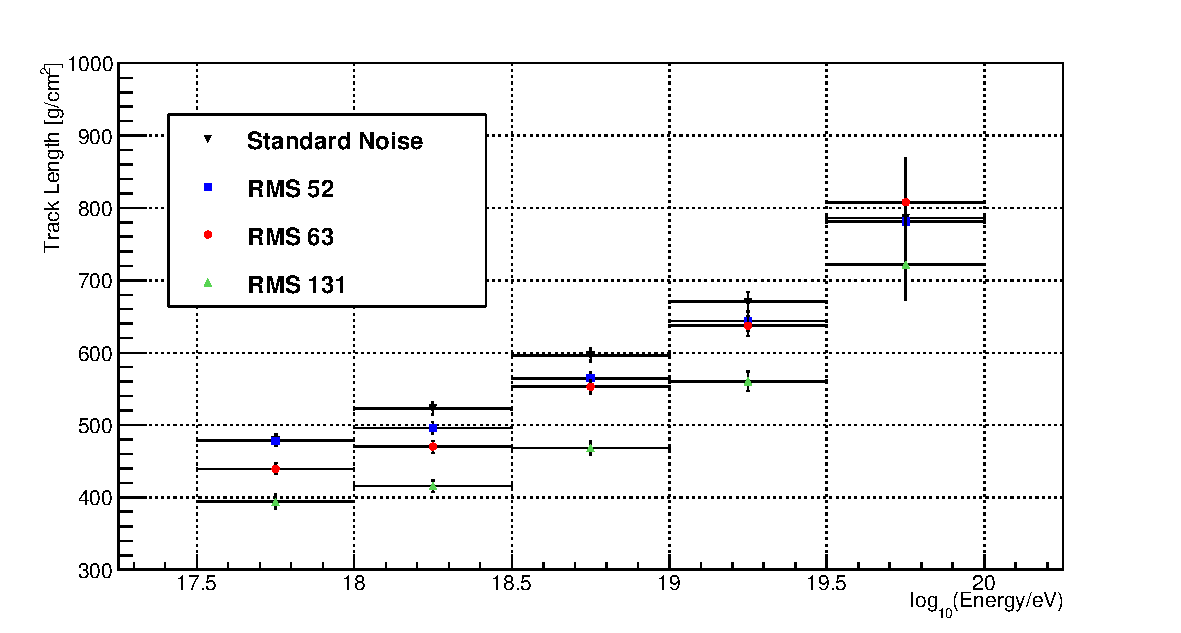
\includegraphics[width=\textwidth]{chapters/graphs/SelectionEff/Smearing_TrackLength_DiffNSBlevels.pdf}
\caption{Track length using Smearing method.} \label{fig:TrackLength_Smearing}
\vspace{3mm}
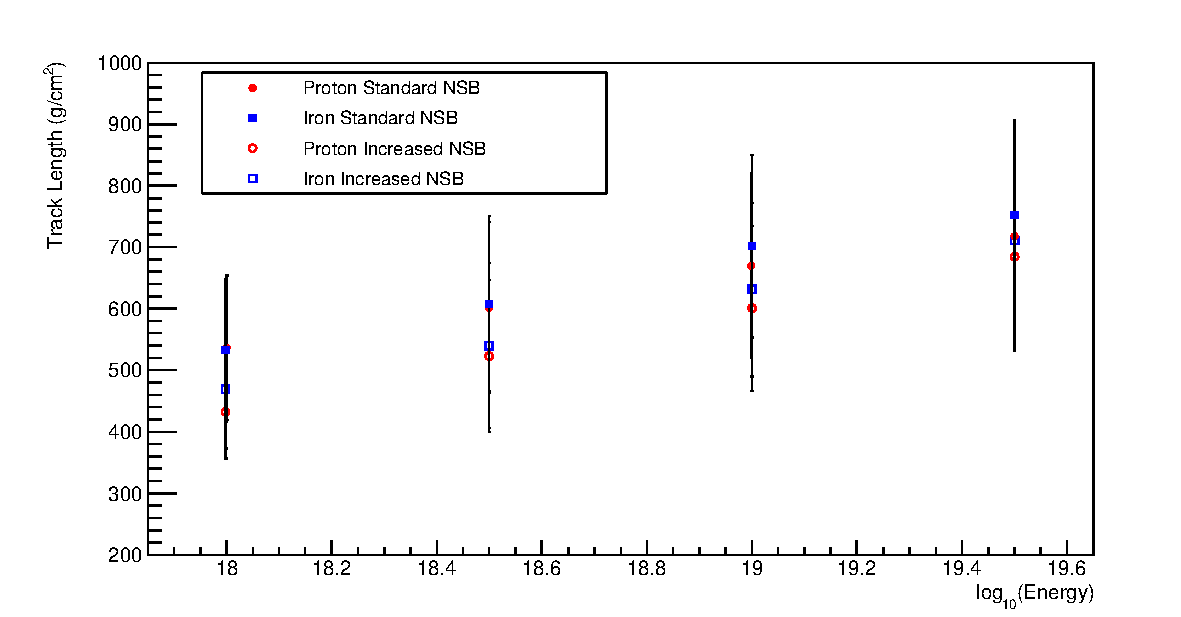
\includegraphics[width=\textwidth]{chapters/graphs/SelectionEff/Simulation_TrackLength_Comb_StandANdIncreasedNSB.pdf}
\caption{Track length using simulation of proton and iron CONEX showers.} \label{fig:TrackLength_Sim}
\end{figure}

%\input{chapters/}
%\input{chapters/}
%\input{chapters/}

\chapter[Conclusion]{\centering Conclusion \\} \label{Ch:Conclusion}
  

\section{Future Work}



\begin{appendices}
%\input{appendix/}
%\input{appendix/}
%\input{appendix/}
%\input{appendix/}
\end{appendices}

\bibliographystyle{ieeetr}
\bibliography{PhD_PaperBiblography}

\end{document}